\chapter{Related Work}
\label{chapter:Related_Work}

\begin{figure}[h!]
  \caption{A picture of a gull.}
  \centering
    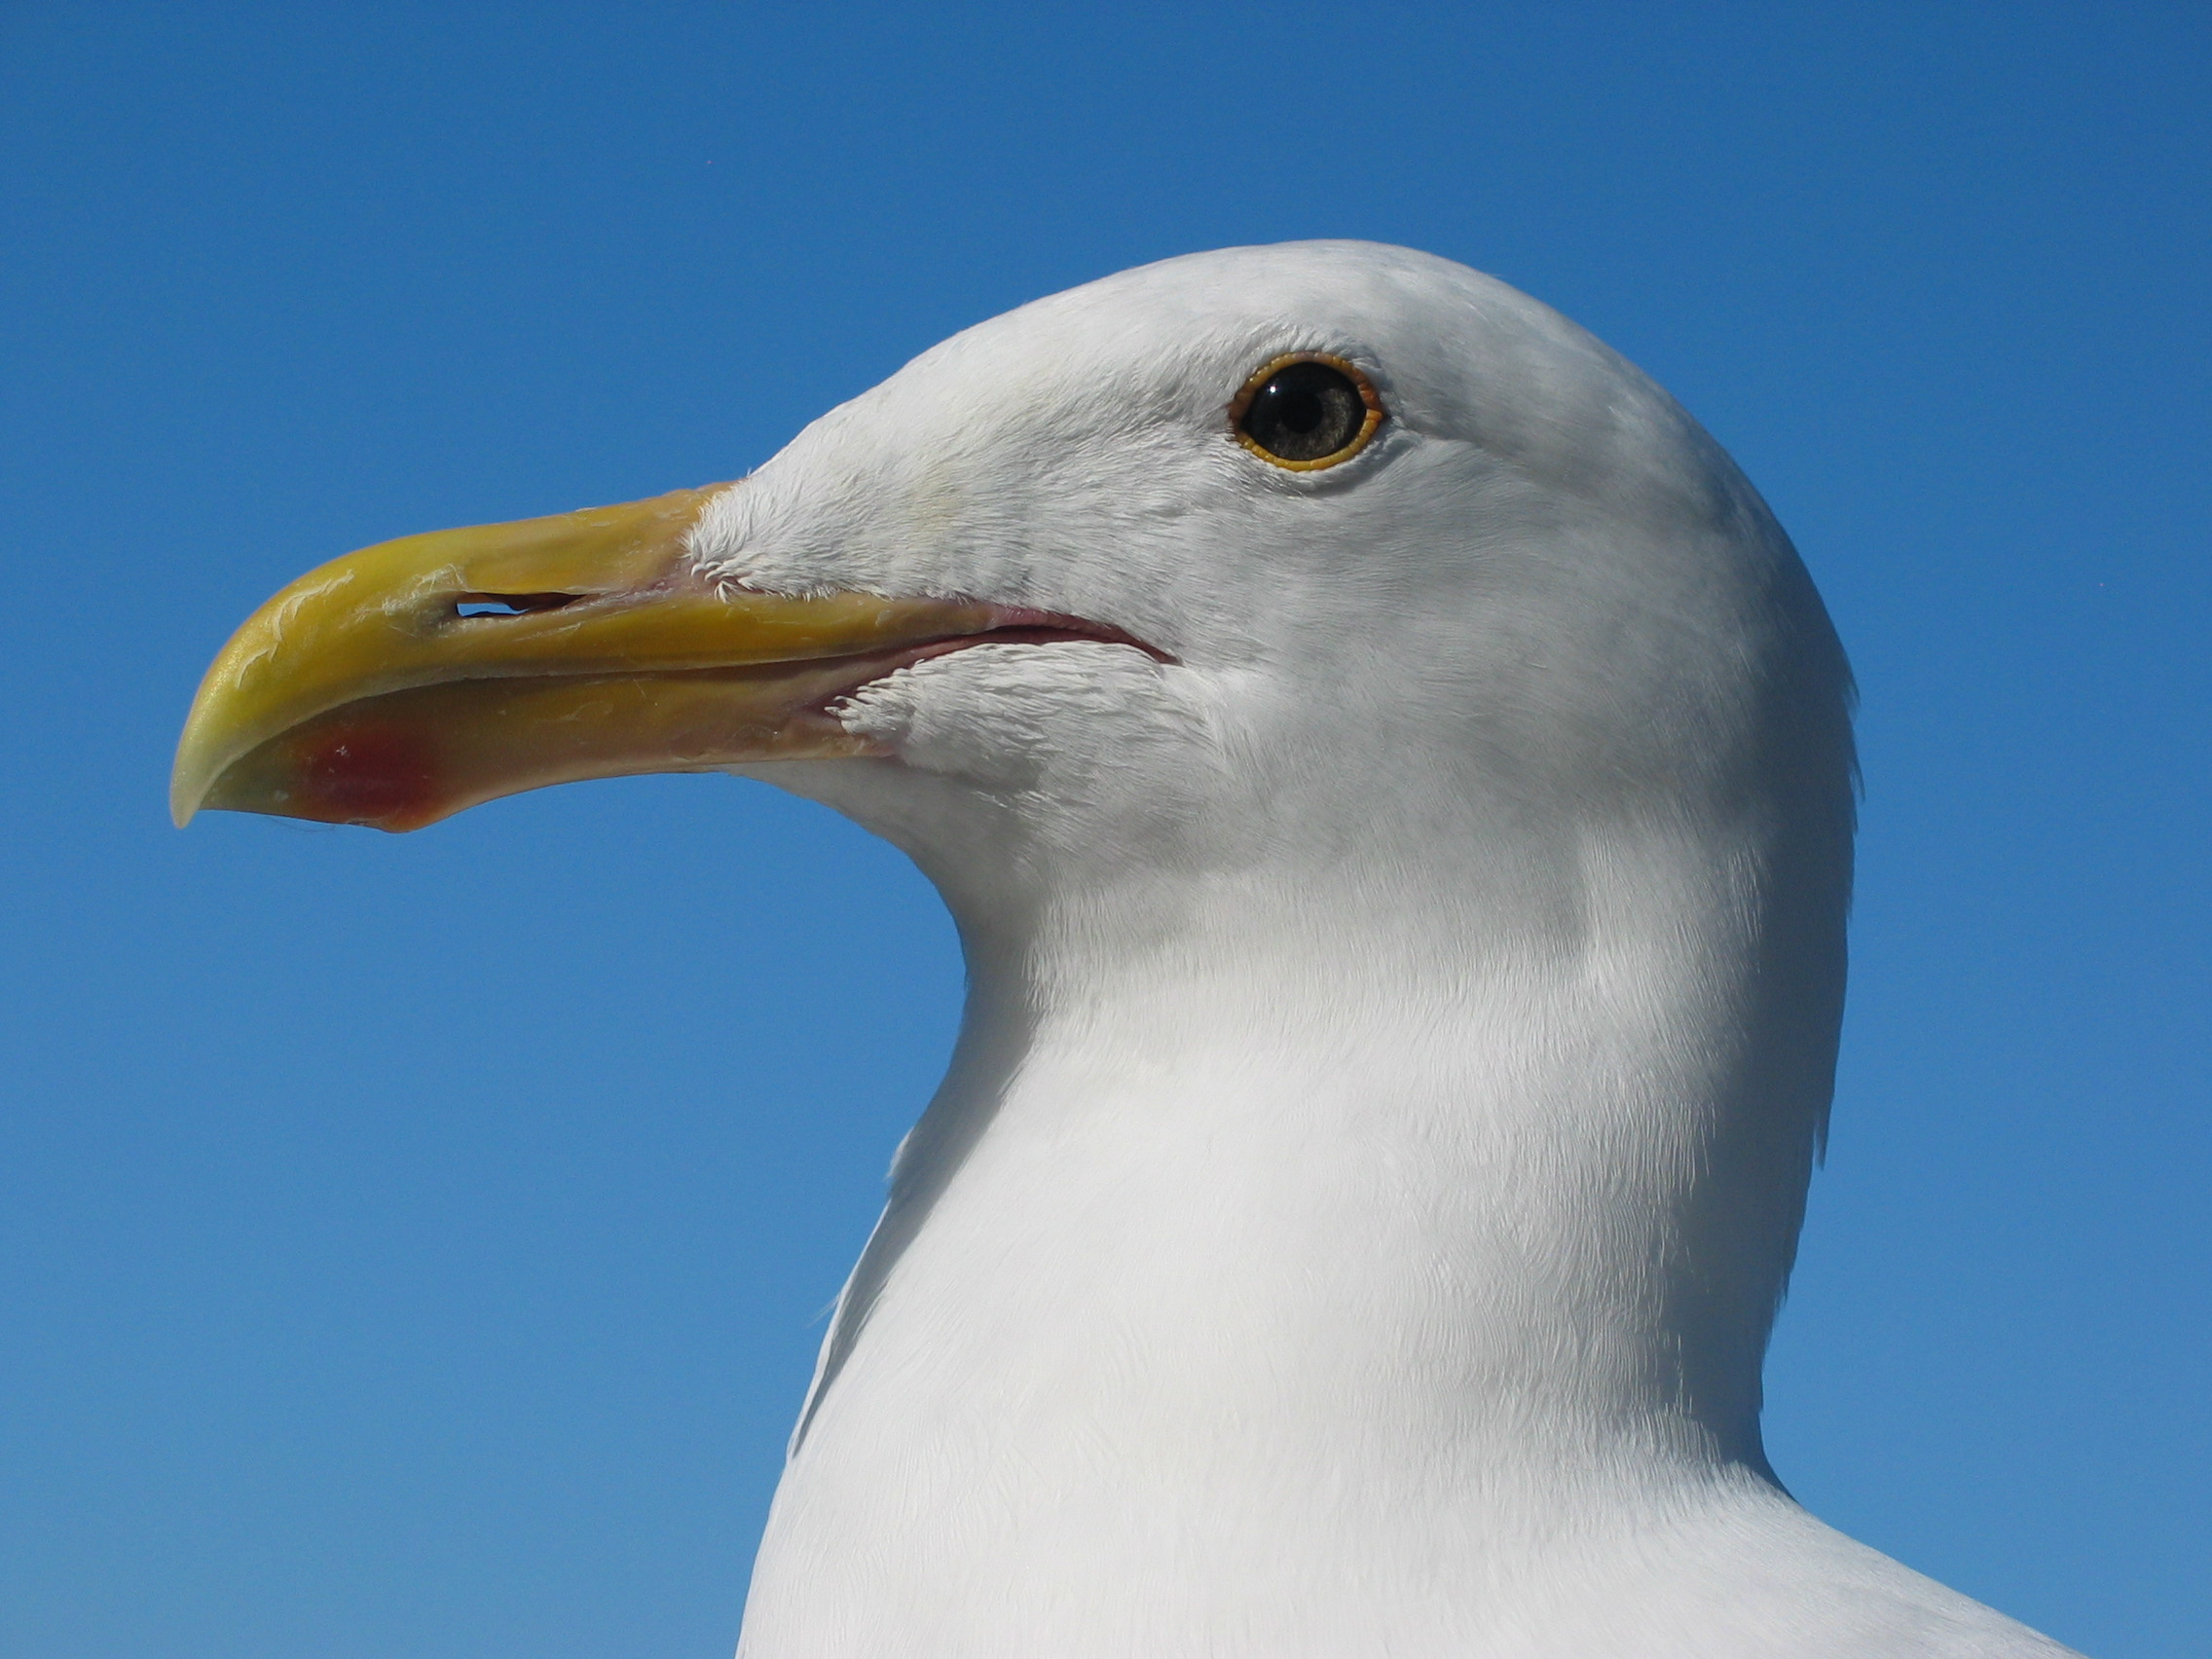
\includegraphics[width=0.8\textwidth]{chapters/images/gull}
\end{figure}

\section{3D geometry}

Yes  - do coordinate systems, transformations, notation
Brief description of SE(3) and SO(3)

\section{Camera Models}

In order to utilise a camera as a sensor, a mapping between image coordinates and world
coordinates needs to be derived.  This allows observations of the camera to be transformed into
meaningful measurements.  To achieve this mapping a sensor model of the camera is required. This
section will cover all the different types of cameras used in this work and corresponding camera
models for each. 

\subsection{Pinhole Camera Model}

The pinhole camera model is the most basic and common of camera models used in computer vision.  It
describes the mathematical relationship between the coordinates of a 3D point in the world and its
projection onto an image plane.  This model assumes the aperture of the camera to be an ideal
pinhole. It does not consider lenses used to focus light which in reality result in lense
distortion.  It does also not take into account sensor quantization apparent in using a modern
digital CCD sensor. Nevertheless it still provides a sufficient model of camera projection for this
work, and practical considerations such as image size, resolution and lense distortion can be
compensated for.

When using the pinhole camera model, the camera is assumed to be a sealed box with a pinhole
aperture on one side, and the image plane, or image sensor on the other side.  Having a small
aperture blocks most of the light rays from objects in the world and allows a focused and inverted
image of the world to be recorded. In this case the focal point is the aperture and the focal length
is the distance from the aperture to the sensor. fig. whatever. For all intensive purposes,
this model can be redrawn as in fig. whatever whatever. The image plane is inverted and shown
reflected in front the of the camera.  As long as the focal length can be determined, it is then
trivial to calculate coordinates on the sensor for a given ray or world coordinate using simple
geometry. Sensor coordinates can then be converted to image coordinates given the physical size
of the CCD and its resolution.  

Take note the principle point is often not in the sensor of the image, and therefore the
coordinates of this point on the sensor needs to be determined.  In addition the focal length
varies from camera to camera and therefore both of these values need to be determined by performing
an intrinsic calibration. For the calibration, the focal length may be expressed in pixel units,
which means the conversion from metric sensor coordinates ( m) to pixel coordinates (u,v) is
also performed in one step.

%http://www.jordicenzano.name/projects/2D-to-3D-Paradigm-overview/camera-model
%use this for picture motivation

\begin{figure}[h!]
  \centering
    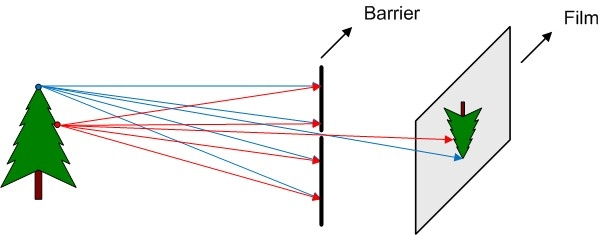
\includegraphics[width=0.5\textwidth]{chapters/images/cam_model_fig2}
  \caption{Pinhole camera model}
\end{figure}

\begin{figure}[h!]
  \centering
    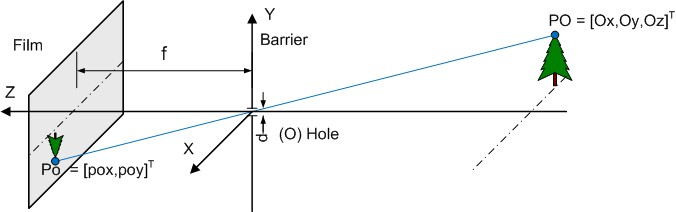
\includegraphics[width=0.9\textwidth]{chapters/images/cam_model_fig41} \\
    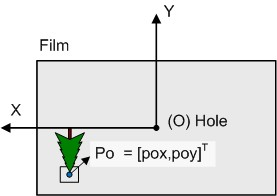
\includegraphics[width=0.3\textwidth]{chapters/images/cam_model_fig42} \\
    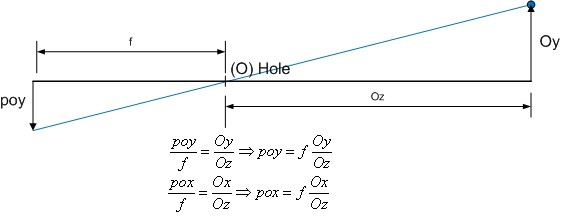
\includegraphics[width=0.9\textwidth]{chapters/images/cam_model_fig43} 
  \caption{Pinhole camera model with image plane shown inverted in front of the focal point}
\end{figure}

%%TODO: I stole these pictures.  I want to redraw them myself

\subsection{Lense Distortion}

The problem with using a pinhole camera in practice is that it does not allow enough light to into
the camera, requiring longer exposure time and therefore blurring in the presence of movement. 
Therefore a double convex lense is used to focus more light rays onto the sensor and allowing a
sharper image.  Such as setup can be seen in fig. xyz.  The pinhole camera model may still be used,
however now lense distortion needs to be accounted for.  Lense distortion causes lines to be
curved, as in fig x.  It is also possible during the intrinsic calibration to simultaneously
determine distortion coefficients which allow the image to be reshaped such that all straight lines
appear straight.

\begin{figure}[h!]
  \centering
    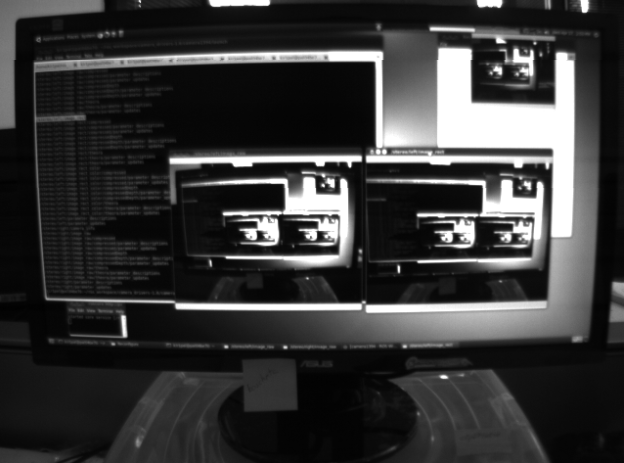
\includegraphics[width=0.49\textwidth]{chapters/images/distorted}
    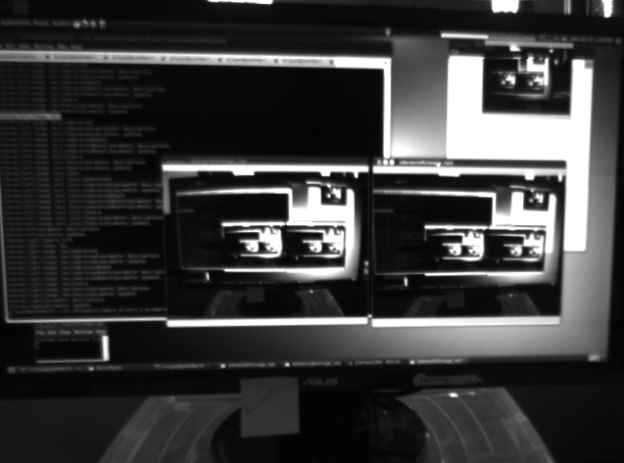
\includegraphics[width=0.49\textwidth]{chapters/images/undistorted}
  \caption{Left: An image with lense distortion.  Right: The same image with lense distortion
compensated for}
\end{figure}

\subsection{Homogeneous coordinates}

%%TODO: homogeneous coords

\begin{equation}
 \begin{pmatrix}
  u \\
  v \\
  1 
 \end{pmatrix} =
 \begin{pmatrix}
  f_x & 0 & c_x \\
  0 & f_y & c_y \\
  0 & 0   & 1 
 \end{pmatrix}
 \begin{pmatrix}
  X \\ Y \\ Z
 \end{pmatrix}
\end{equation}


\subsection{Stereo Camera}

\subsection{Omni-directional Camera}

\subsection{Flir}
Leave this to last.  Flir may (probably) get left out

\section{Computer Vision Basics}

\subsection{Feature point detection and extraction}

Outline what is feature point detection, description and matching, why we need
it.  Mention SIFT
and SURF and cite them.  Mention that we used a GPU implemtation of SIFT, cite
the ETH paper. 
Mention a bunch of other descriptors, cite them as well.

\subsection{RANSAC}

explain this cos its easy and fun.  Cite a paper

\subsection{Geometry estimation}

\subsubsection{5 point algorithm}

ask for matthias for relavent literature

\subsubsection{Point triangulation}

ask for matthias for relavent literature

\subsubsection{Stereo pose estimation}

Umeyama (PCL) \newline 
Horn (UVM)


\section{Place Recognition}

Bag of words

\section{Visual SLAM}

Cover this in abstract terms.  Talk about the theory, not implemtation.  Mention
PTAM and cite it.
No g2o here.

\subsection{Keyframe SLAM}

\subsection{Graph SLAM}
